\documentclass[11pt,a4paper]{article}

\usepackage{fontspec}
\usepackage[a4paper,top=2.4cm,bottom=2.4cm,left=2.6cm,right=2.6cm]{geometry}
\usepackage{graphicx}
\usepackage{float}   % [H]: floats stay where they are written, next to their commentary
\usepackage{booktabs}
\usepackage{tabularx}
\usepackage{xcolor}
\usepackage{caption}
\usepackage[hidelinks]{hyperref}

% --- type: the same family as the figures -----------------------------------
\setmainfont{Helvetica Neue}[
  UprightFont = * Light,
  BoldFont    = * Medium,
  ItalicFont  = * Light Italic,
  Scale       = 1.0
]
\newfontfamily\headingfont{Helvetica Neue}[UprightFont = * Medium]

% --- colours: the project's validated palette --------------------------------
\definecolor{ink}{HTML}{0B0B0B}
\definecolor{inksec}{HTML}{52514E}
\definecolor{inkmuted}{HTML}{898781}
\definecolor{rule}{HTML}{E1E0D9}
\definecolor{lightside}{HTML}{2A78D6}
\definecolor{darkside}{HTML}{E34948}

\color{ink}
\setlength{\parindent}{0pt}
\setlength{\parskip}{0.62em}
\linespread{1.12}

% --- section headings (titlesec is absent from this TeX installation) --------
\newcommand{\heading}[1]{%
  \penalty-150\vspace{1.5em}%
  {\headingfont\fontsize{13.5}{16}\selectfont\color{ink}#1}\\[0.35em]%
  {\color{rule}\rule{\linewidth}{0.7pt}}\\[0.15em]%
  \nopagebreak}

\newcommand{\subheading}[1]{%
  \vspace{0.5em}%
  {\headingfont\fontsize{11}{13}\selectfont\color{inksec}#1}\\[0.1em]%
  \nopagebreak}

\newcommand{\lead}[1]{{\color{inksec}\fontsize{10.5}{14}\selectfont #1}\par}

\captionsetup{font={small,color=inkmuted},labelfont={color=inksec},skip=6pt}

\begin{document}
\pagestyle{plain}

% ============================ HEADER ========================================
{\headingfont\fontsize{22}{26}\selectfont
Did Anakin Skywalker's language\\[0.15em]
actually change?\par}

\vspace{0.6em}
{\color{inksec}\fontsize{12}{15}\selectfont
Measuring a character's turn to the dark side from screenplay dialogue alone\par}

\vspace{1.2em}
{\color{inkmuted}\small Samuel Ballu \quad·\quad Python, scikit-learn, PyTorch, Transformers\par}

\vspace{0.4em}
{\color{rule}\rule{\linewidth}{1.2pt}}

\vspace{1.2em}

\begin{figure}[H]
\centering
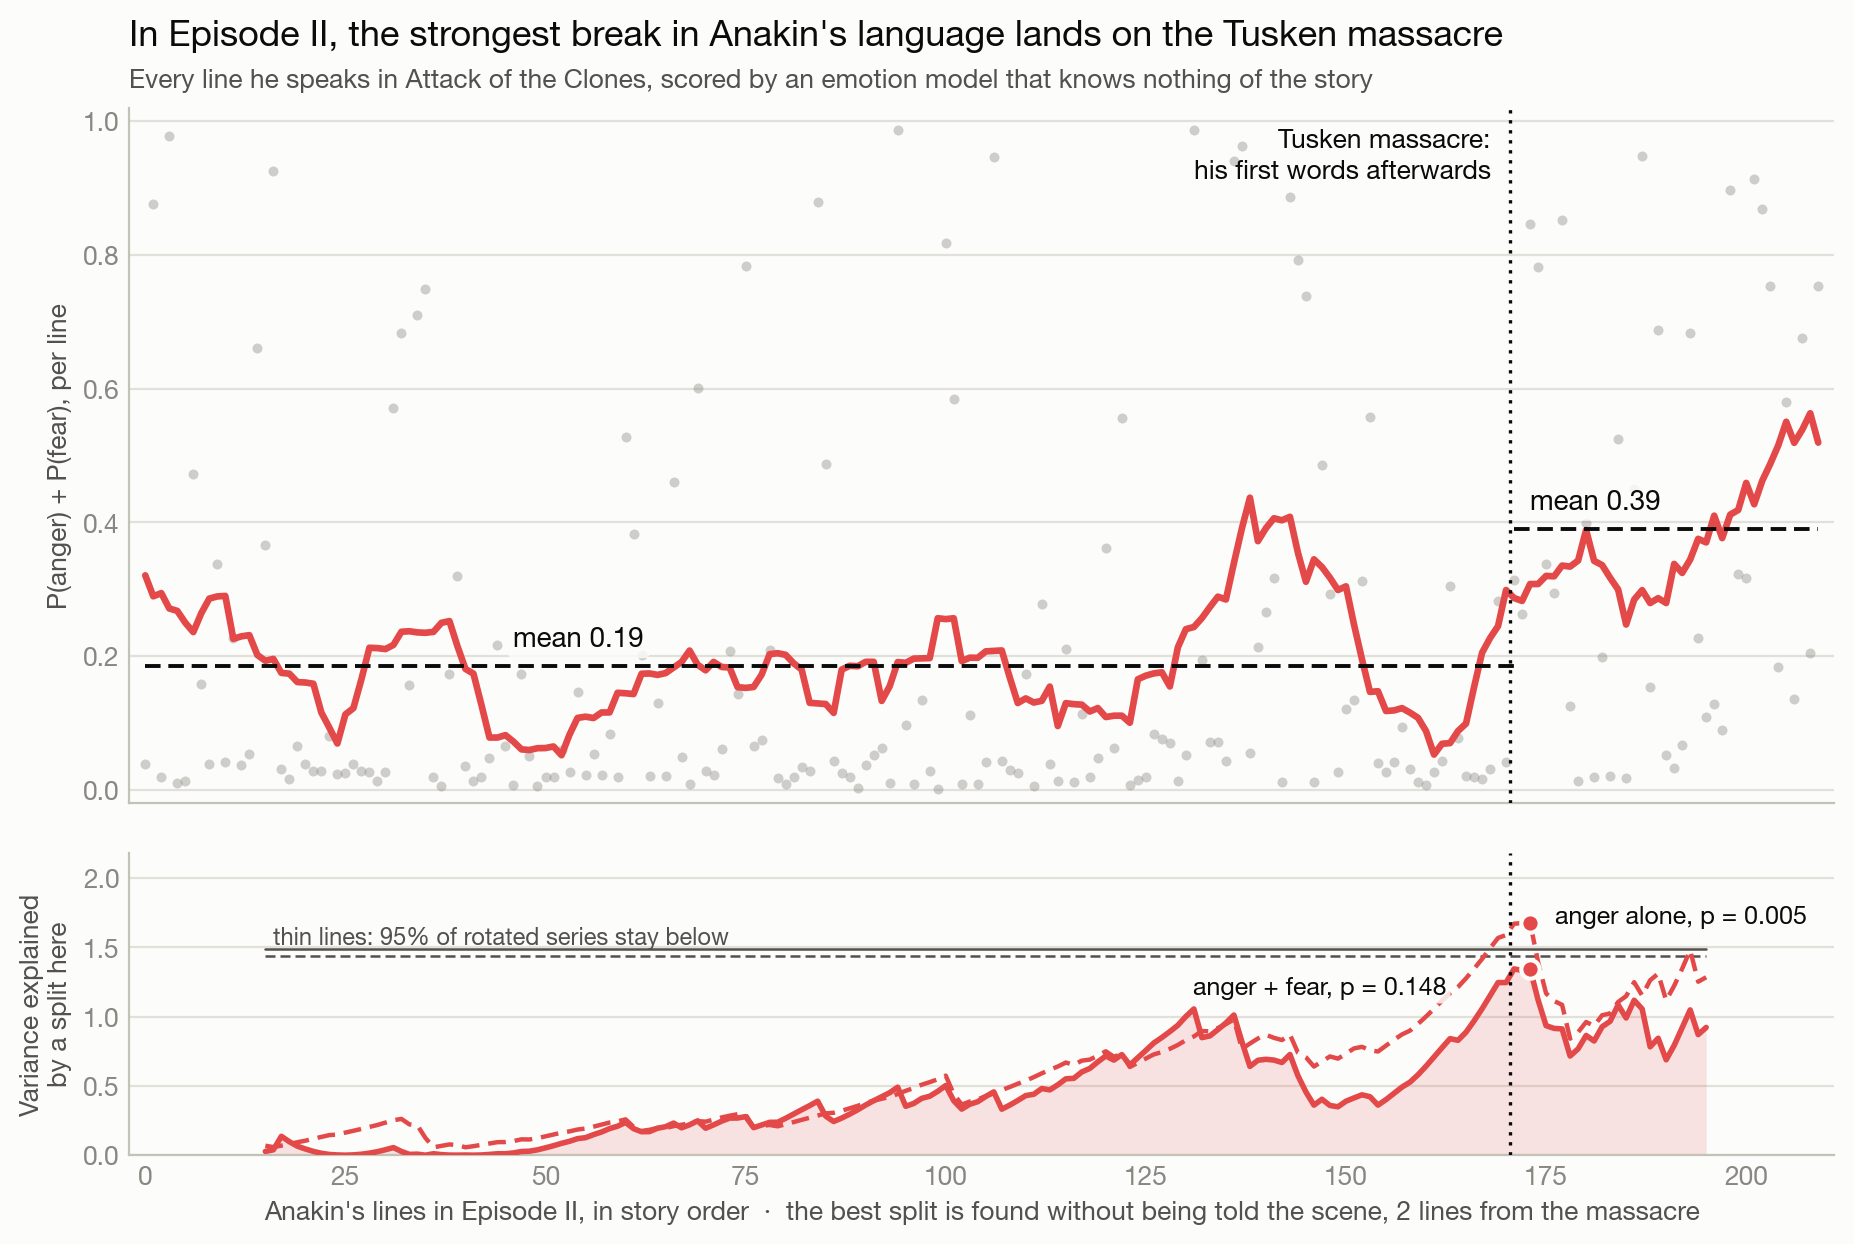
\includegraphics[width=\linewidth]{../figures/00_tusken_break.png}
\end{figure}

\vspace{0.6em}

\lead{During my master's in statistics and artificial intelligence I built an NLP project
on Star Wars: scrape the screenplays of Episodes~I to~III and try to detect Anakin
Skywalker's turn to the dark side from his dialogue alone. The classifier reported 77~\%
accuracy, and a curve showed a gradual descent.}

\lead{I rebuilt it. Neither result held up, because of how the model was evaluated and how
the curve was plotted. Once that is fixed, his language does change, but not at one single
moment. Inside Episode~II the strongest break lands on the massacre of the Tusken camp. It
does not last, and across the whole trilogy the largest breaks come later, in Episode~III.}

% ============================ 1 =============================================
\heading{1. What was wrong: the split}

The label ``light side'' or ``dark side'' belongs to a \textbf{character}, not to a sentence.
The original split its lines at random between training and test, so Yoda appeared on both
sides. A model could then score by learning how Yoda talks, without learning anything about
the two camps. That skill is worth nothing on a character it has never seen, and Anakin is
never in training.

The rebuild uses a \texttt{StratifiedGroupKFold} grouped by character: all of a character's
lines are in training or all are in test. The random split stays in the code so that the gap
can be measured.

\begin{figure}[H]
\centering
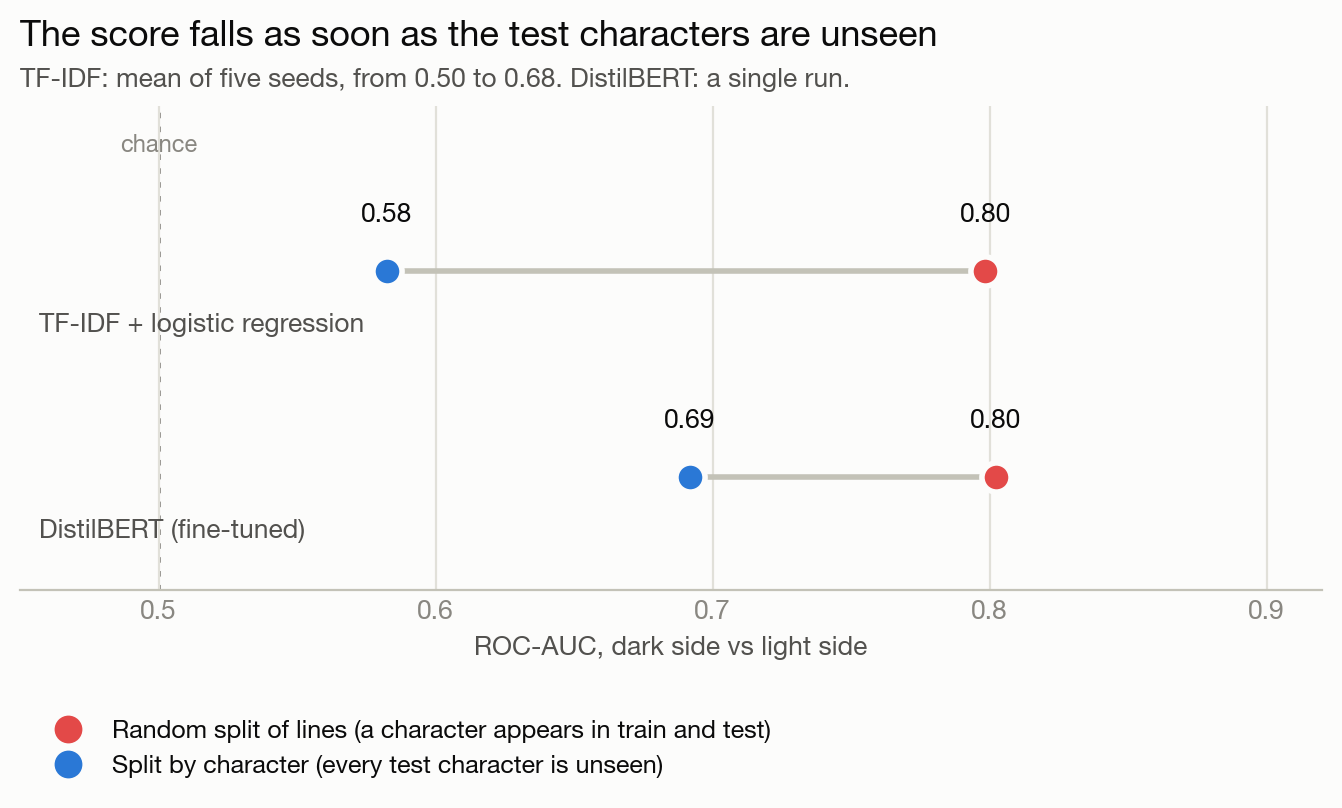
\includegraphics[width=0.9\linewidth]{../figures/01_validation_gap.png}
\caption{Same data, two validation protocols.}
\end{figure}

TF-IDF falls from ROC-AUC 0.80 to 0.58 on average, and the five seeds run from 0.50 to 0.68
depending on which characters share a fold. With seven dark-side characters, that spread is
itself a result.

\subheading{DistilBERT shows no demonstrated gain}

The 0.69 and 0.58 in the figure should not be compared directly, because DistilBERT ran once.
On identical folds the two models score 0.69 and 0.68. Without Palpatine, TF-IDF scores higher
(0.68 against 0.60).

\begin{figure}[H]
\centering
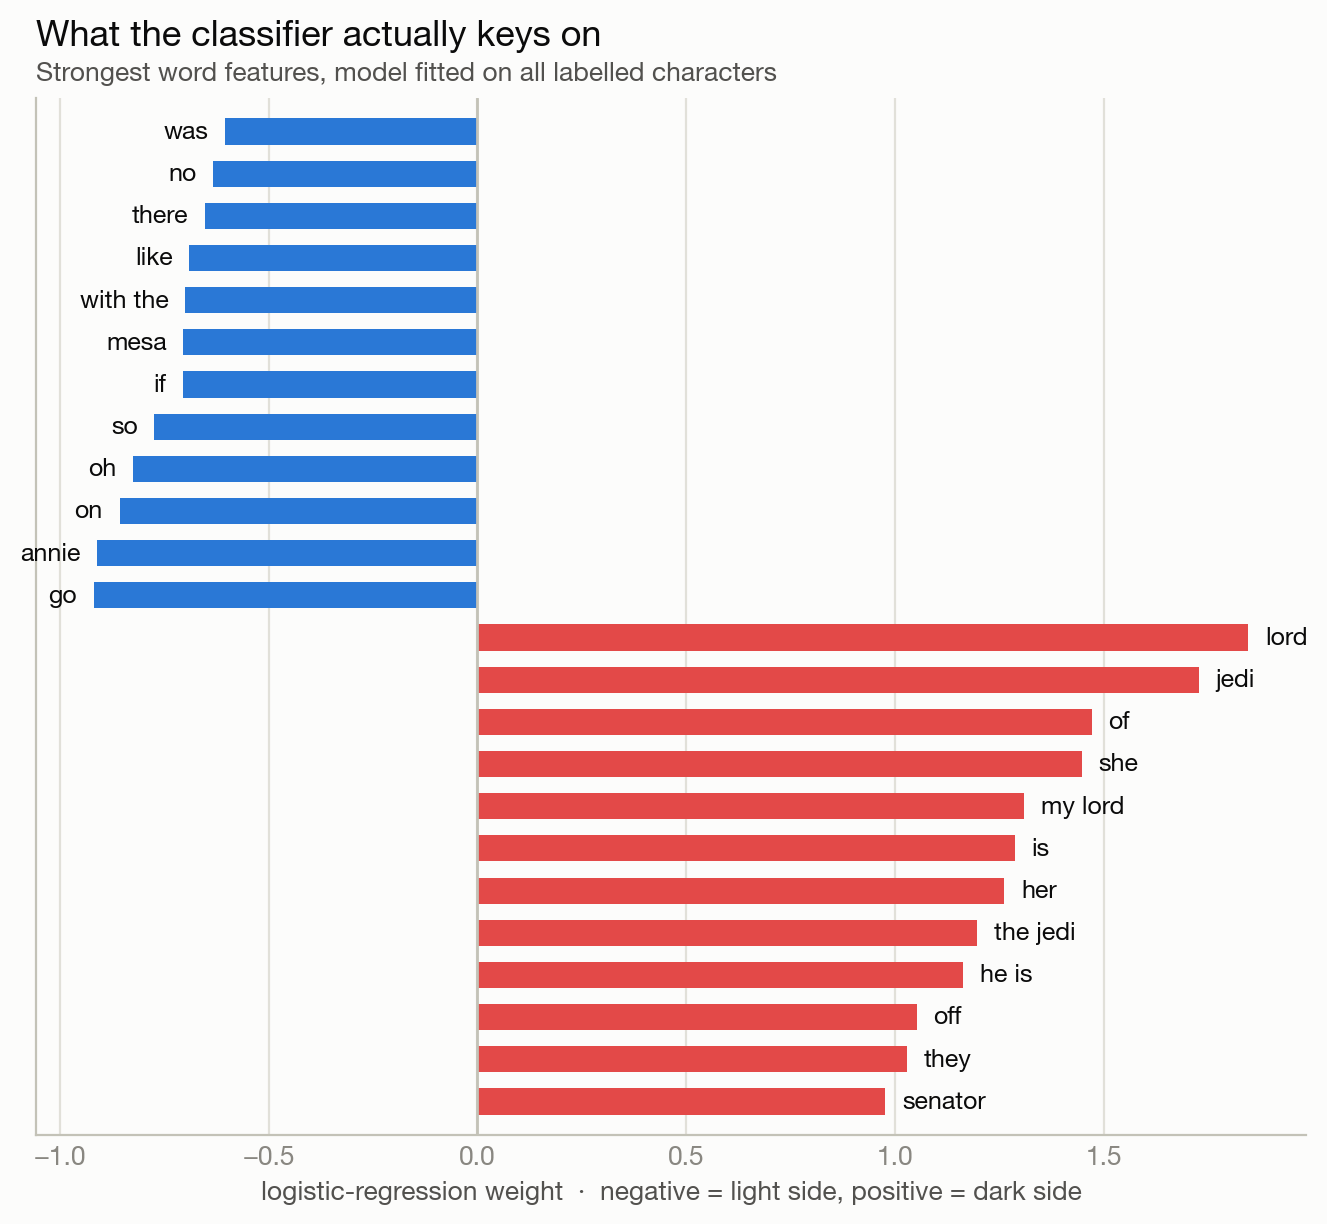
\includegraphics[width=0.56\linewidth]{../figures/04_top_terms.png}
\caption{The strongest word features. \emph{mesa} is almost entirely Jar Jar's, and
\emph{annie} is the nickname other characters use for Anakin.
Neither says anything about the rhetoric of a camp.}
\end{figure}

% ============================ 2 =============================================
\heading{2. What was wrong: the curve}

The headline figure counted ``evil'' lines cumulatively:

\vspace{-0.3em}
\begin{center}
\texttt{\small if prediction == 'mechant': compteur += 1}
\end{center}
\vspace{-0.3em}

A running count can only rise, so a rising curve showed nothing about a fall. The rebuild works
on levels and tests every claim against a null model:

\begin{itemize}
\setlength\itemsep{0.15em}
\item \textbf{p-values come from rotation tests.} The series is circularly shifted against story
      time, for every possible shift. Neighbouring lines are correlated, and shuffling them one
      by one would give p-values that are too small. The smallest reachable value is $1/n$.
\item \textbf{Confidence intervals resample scenes} rather than lines, for the same reason.
\end{itemize}

% ============================ 3 =============================================
\newpage
\heading{3. The other fixes}

\begin{table}[H]
\small
\begin{tabularx}{\linewidth}{lXX}
\toprule
 & \textbf{Original} & \textbf{Rebuild} \\
\midrule
Names &
\texttt{SequenceMatcher} at 0.8 on every uppercase token. It fixed real typos (\texttt{ANKAIN})
but also turned \texttt{MACE} into \texttt{MENACE} and \texttt{KNIGHT} into \texttt{NIGHT} &
Explicit alias table, read off the real cue frequencies \\
\addlinespace
Text &
Punctuation removed before analysis &
Punctuation and casing kept \\
\addlinespace
Labels &
Two ChatGPT-generated lists, with names cut short by the regex (\texttt{TEY HOW} became
\texttt{HOW}) and most antagonists counted as dark side &
Curated camps; 12 characters left unlabelled, each with a recorded reason \\
\addlinespace
Same person &
\texttt{AMIDALA} and \texttt{PADME} kept apart &
Personas merged: Padm\'e/Amidala, Palpatine/Sidious, Anakin/Vader \\
\addlinespace
Sentiment &
TextBlob polarity on stripped text &
7-way emotion model on clean text \\
\bottomrule
\end{tabularx}
\end{table}

The emotion model (\texttt{emotion-english-distilroberta-base}) was trained elsewhere and knows
nothing of Star Wars or of this project's labels. The main indicator, \texttt{P(anger) + P(fear)},
was chosen from the saga's own stated chain before any line was scored. This was not a formal
pre-registration.

% ============================ 4 =============================================
\heading{4. The Tusken massacre}

Anakin says nothing during the massacre. His first words afterwards are in the homestead garage
(Episode~II, scene~125), so that is where it can first show in dialogue. The figure on the first
page shows every line of the episode. Its lower panel is computed without being told where the
massacre is.

\begin{table}[H]
\centering
\small
\begin{tabularx}{\linewidth}{Xccccc}
\toprule
\textbf{Episode II only} & \textbf{Before} & \textbf{After} & \textbf{Step p} & \textbf{Blind split} & \textbf{Blind p} \\
\midrule
P(anger) + P(fear) & 0.185 & 0.391 & 0.010 & 2 lines after & 0.148 \\
P(anger) alone & 0.088 & 0.318 & 0.005 & 2 lines after & 0.005 \\
P(dark side), DistilBERT & 0.059 & 0.269 & 0.034 & 1 line after & 0.080 \\
P(dark side), TF-IDF & 0.279 & 0.339 & 0.045 & 1 line before & 0.386 \\
\bottomrule
\end{tabularx}
\caption{``Step'' tests a rise at the massacre. ``Blind'' searches every split with at least 15
lines on each side and asks whether a split that good appears by chance.}
\end{table}

\subheading{What supports it}

All four measures rise at the massacre, and all four blind searches land within 2 lines of it.
The rise does not rest on the garage scene alone: without it, the after-massacre mean of
\texttt{P(anger) + P(fear)} is still 0.369, and 0.286 once the angriest later scene (the gunship,
scene~164) is removed as well.

\subheading{What limits it}

\begin{itemize}
\setlength\itemsep{0.15em}
\item The location is a best estimate. When scenes are resampled, the break lands on scene~125 in
      28~\% of runs, and the 90~\% interval runs from scene~21 to scene~164.
\item Only anger clears the bar in the blind search. \texttt{P(anger) + P(fear)}, the measure chosen
      in advance, does not.
\item With a minimum of 5 or 10 lines per side, the emotion measures and DistilBERT move to later
      scenes (the gunship, scene~164, and scene~160).
\item Padm\'e rises at the same point too (anger 0.106 to 0.239), possibly because the war is starting. Anakin's
      jump is larger, but the difference is not statistically clear ($+0.097$, 95~\% CI $-0.085$ to
      $+0.244$). Against Obi-Wan it is clear for anger ($+0.210$, CI $+0.021$ to $+0.340$), not for
      anger + fear ($+0.184$, CI $-0.013$ to $+0.344$).
\item I looked at this scene because of the story and the curves. The location comes from the
      screenplay, but limiting the search to Episode~II was my choice, so this is an informed reading
      rather than a blind discovery.
\end{itemize}

These numbers measure what his dialogue expresses. The moral turn itself is an interpretation.

% ============================ 5 =============================================
\heading{5. Across the whole trilogy}

\begin{figure}[H]
\centering
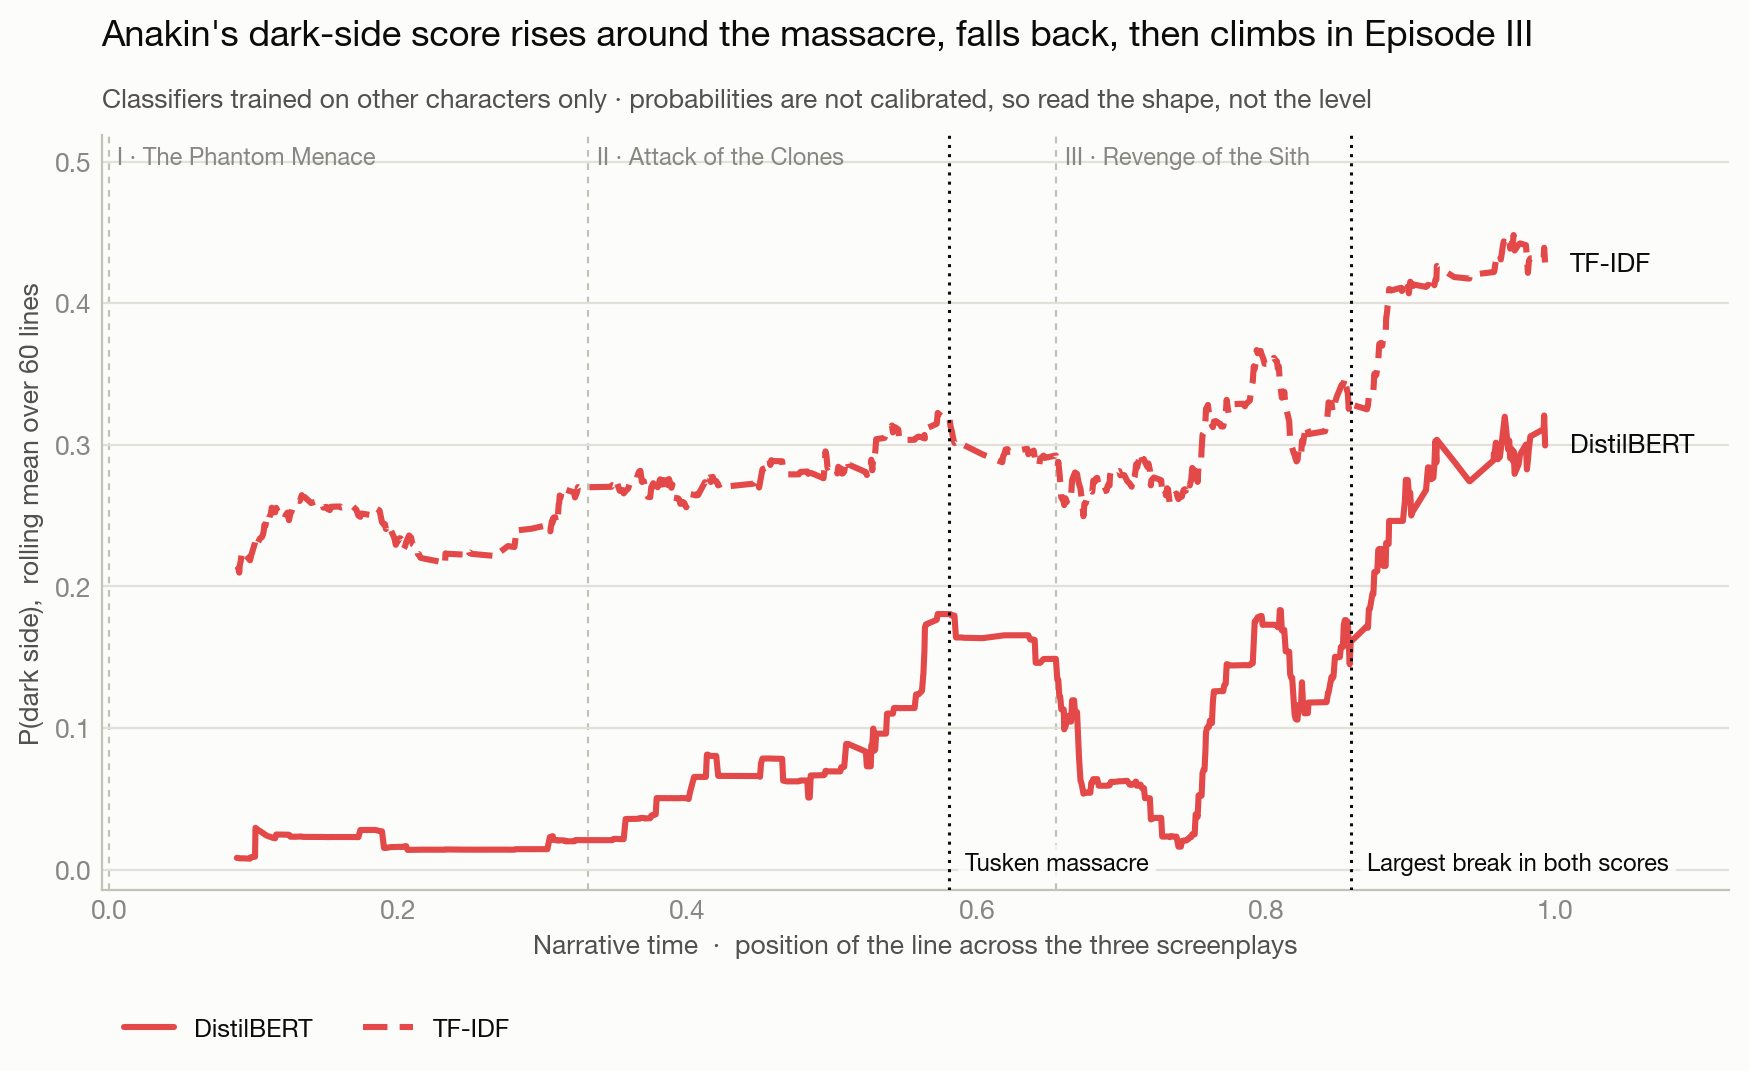
\includegraphics[width=0.94\linewidth]{../figures/06_dark_score.png}
\caption{The score comes from classifiers trained on the other characters only.}
\end{figure}

The dark-side score rises through the trilogy (DistilBERT $\rho = +0.33$, p $= 0.002$; TF-IDF
$\rho = +0.21$, p $= 0.011$). But the massacre break does not last:

\begin{table}[H]
\centering
\small
\begin{tabular}{lcccc}
\toprule
 & \textbf{Before massacre} & \textbf{After, Ep.~II} & \textbf{Ep.~III, 1st half} & \textbf{Ep.~III, 2nd half} \\
\midrule
P(anger) + P(fear) & 0.185 & 0.391 & 0.204 & 0.272 \\
P(dark side), DistilBERT & 0.059 & 0.269 & 0.057 & 0.216 \\
\bottomrule
\end{tabular}
\end{table}

Searching the whole trilogy, both classifiers pick the same line at position 0.86, in Episode~III
(DistilBERT 0.067 to 0.294, p $= 0.003$; TF-IDF 0.275 to 0.429, p $= 0.002$). It falls in scene~103,
just before the Chancellor's office scenes (116 to 130); the script has him kneel in scene~128. The
classifiers may partly be picking up the subject of those conversations rather than a change in
Anakin, since half of the dark-side training lines are Palpatine's.

\begin{figure}[H]
\centering
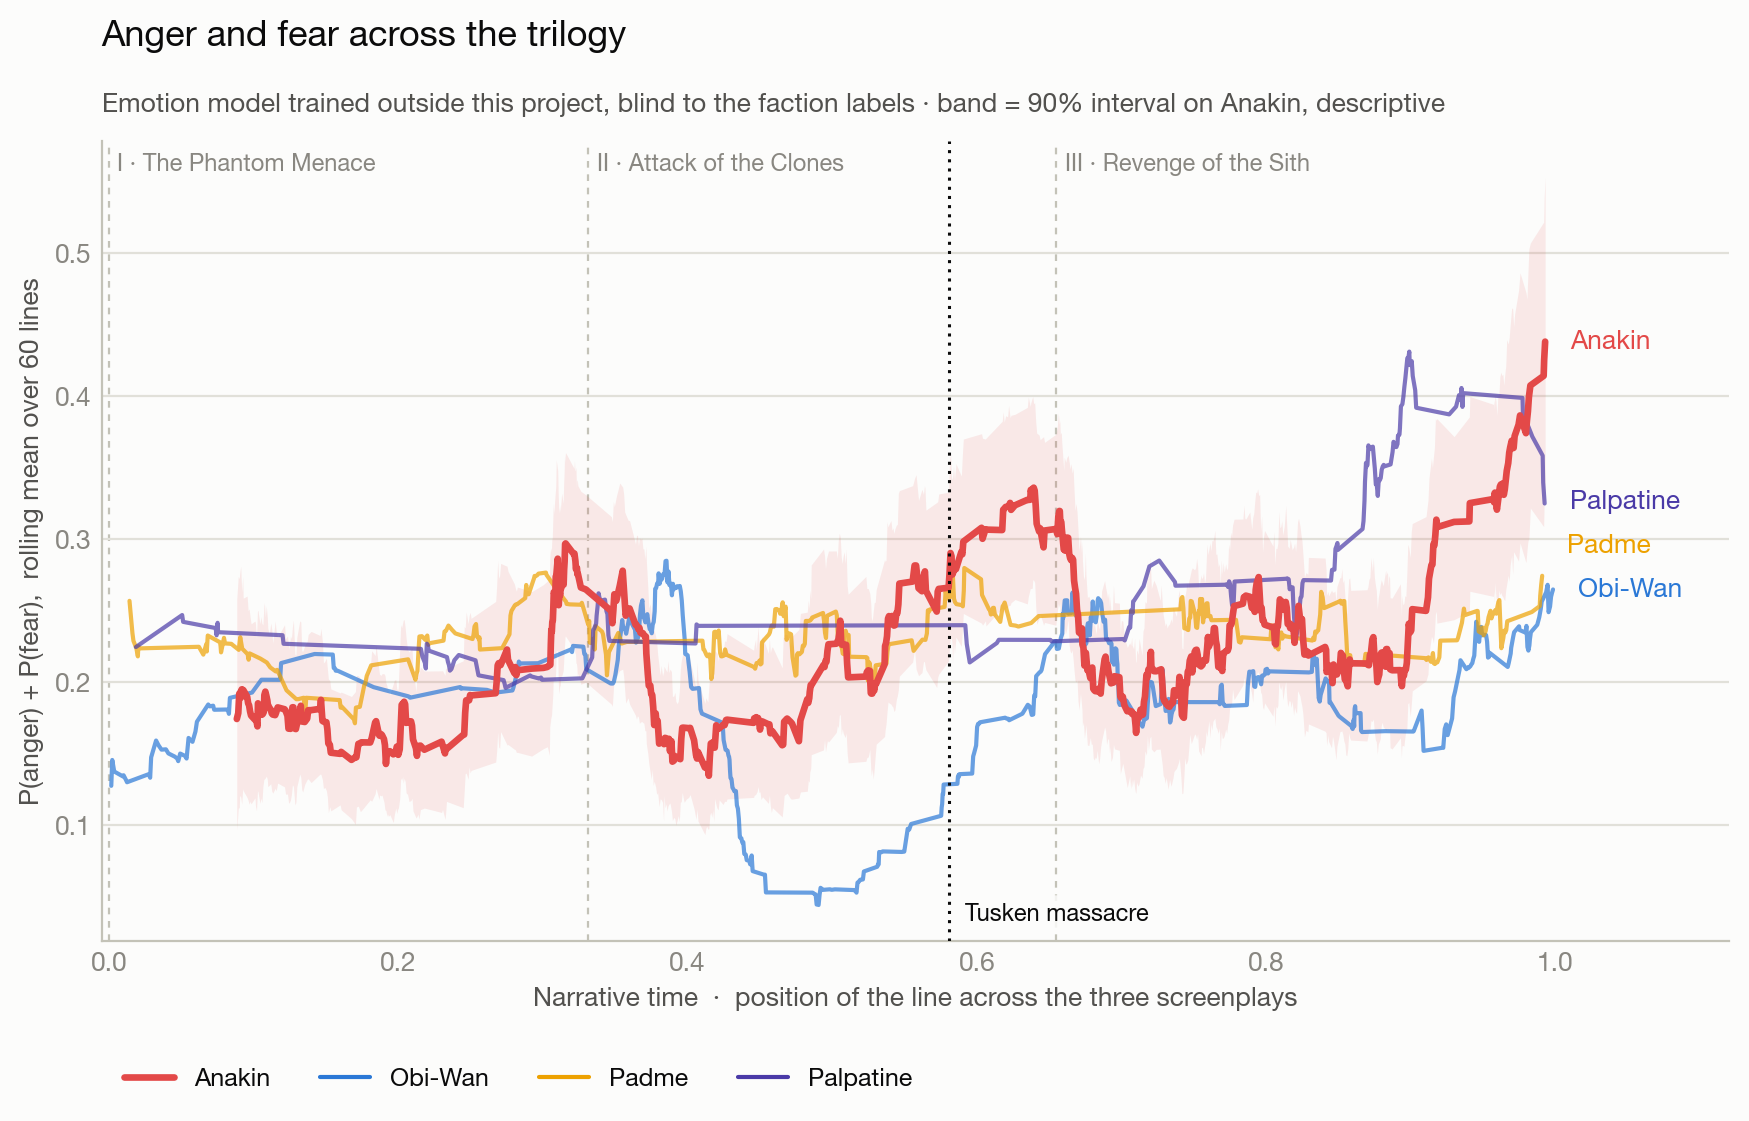
\includegraphics[width=0.94\linewidth]{../figures/02_emotional_arc.png}
\end{figure}

Anger and fear also rise overall ($\rho = +0.129$, p $= 0.006$). A single break for this measure is
not stable: it lands at Mustafar with a minimum of 15 or 30 lines per side (p $= 0.020$ and $0.004$),
and on Naboo with a minimum of 50 (p $= 0.073$).

\begin{table}[H]
\centering
\small
\begin{tabularx}{\linewidth}{Xcc}
\toprule
\textbf{Slope of anger + fear, Anakin minus control} & \textbf{Difference} & \textbf{95\% CI} \\
\midrule
Pooled light side (19 characters) & $+0.103$ & $[-0.009,\,+0.213]$ \\
Obi-Wan & $+0.077$ & $[-0.072,\,+0.216]$ \\
Padm\'e & $+0.111$ & $[-0.031,\,+0.258]$ \\
Palpatine & $-0.083$ & $[-0.278,\,+0.123]$ \\
\bottomrule
\end{tabularx}
\caption{No interval excludes zero, so this overall rise is not clearly his alone.}
\end{table}

\begin{figure}[H]
\centering
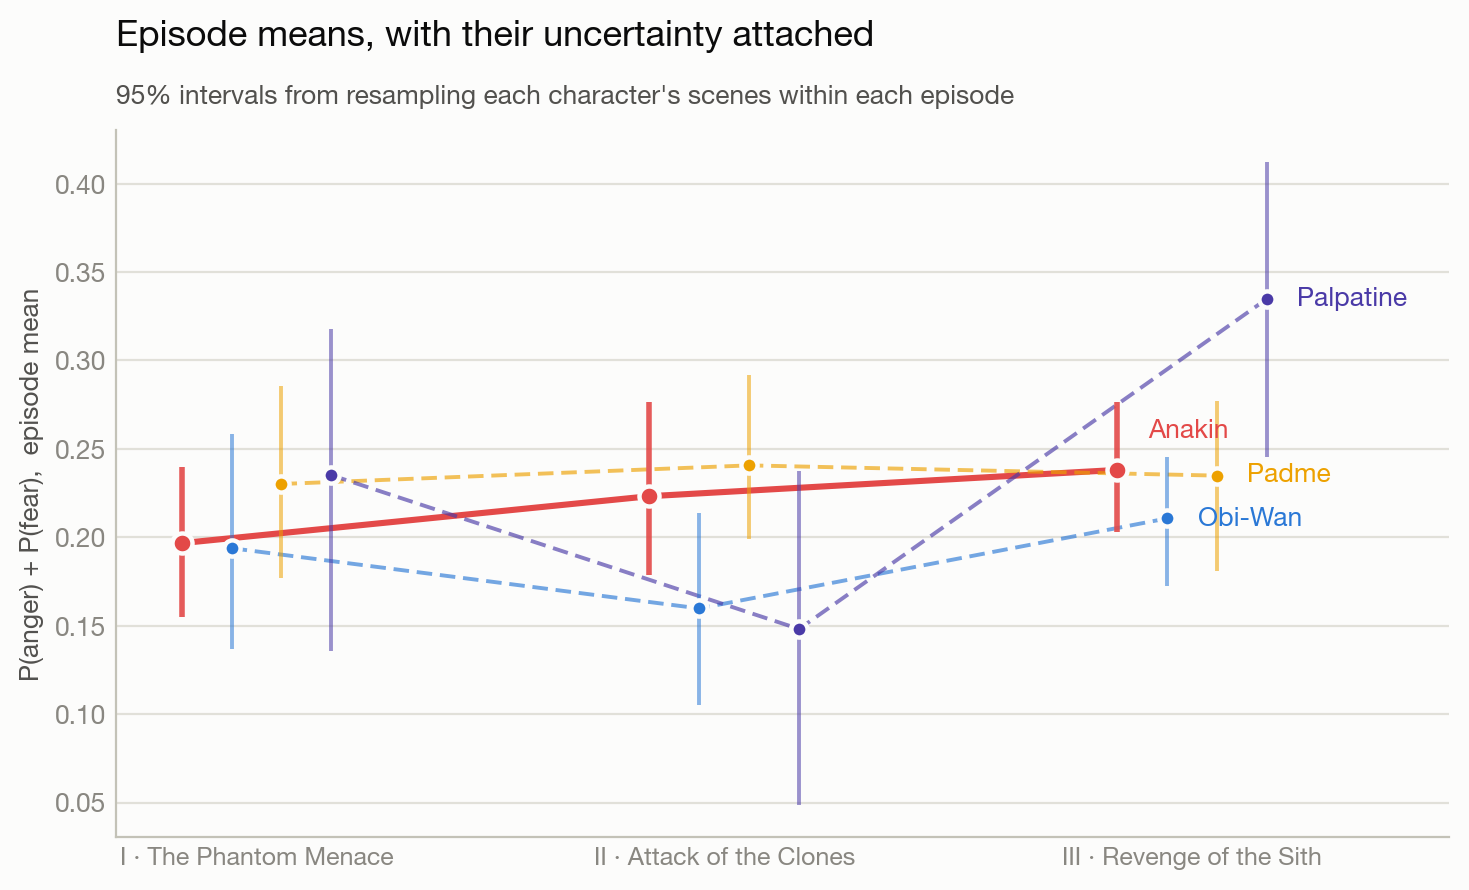
\includegraphics[width=0.66\linewidth]{../figures/05_by_episode.png}
\end{figure}

% ============================ 6 =============================================
\heading{6. Which emotions move}

\begin{table}[H]
\centering
\small
\begin{tabular}{lrrr}
\toprule
\textbf{Emotion} & \textbf{$\rho$} & \textbf{p} & \textbf{p, Holm-adjusted} \\
\midrule
surprise & $-0.234$ & 0.008 & 0.051 \\
joy      & $-0.169$ & 0.006 & 0.039 \\
anger    & $+0.118$ & 0.070 & 0.254 \\
disgust  & $+0.094$ & 0.013 & 0.063 \\
fear     & $+0.085$ & 0.063 & 0.254 \\
neutral  & $+0.063$ & 0.497 & 0.994 \\
sadness  & $-0.034$ & 0.585 & 0.994 \\
\bottomrule
\end{tabular}
\caption{Trend of each emotion in Anakin's dialogue against story time.}
\end{table}

\begin{figure}[H]
\centering
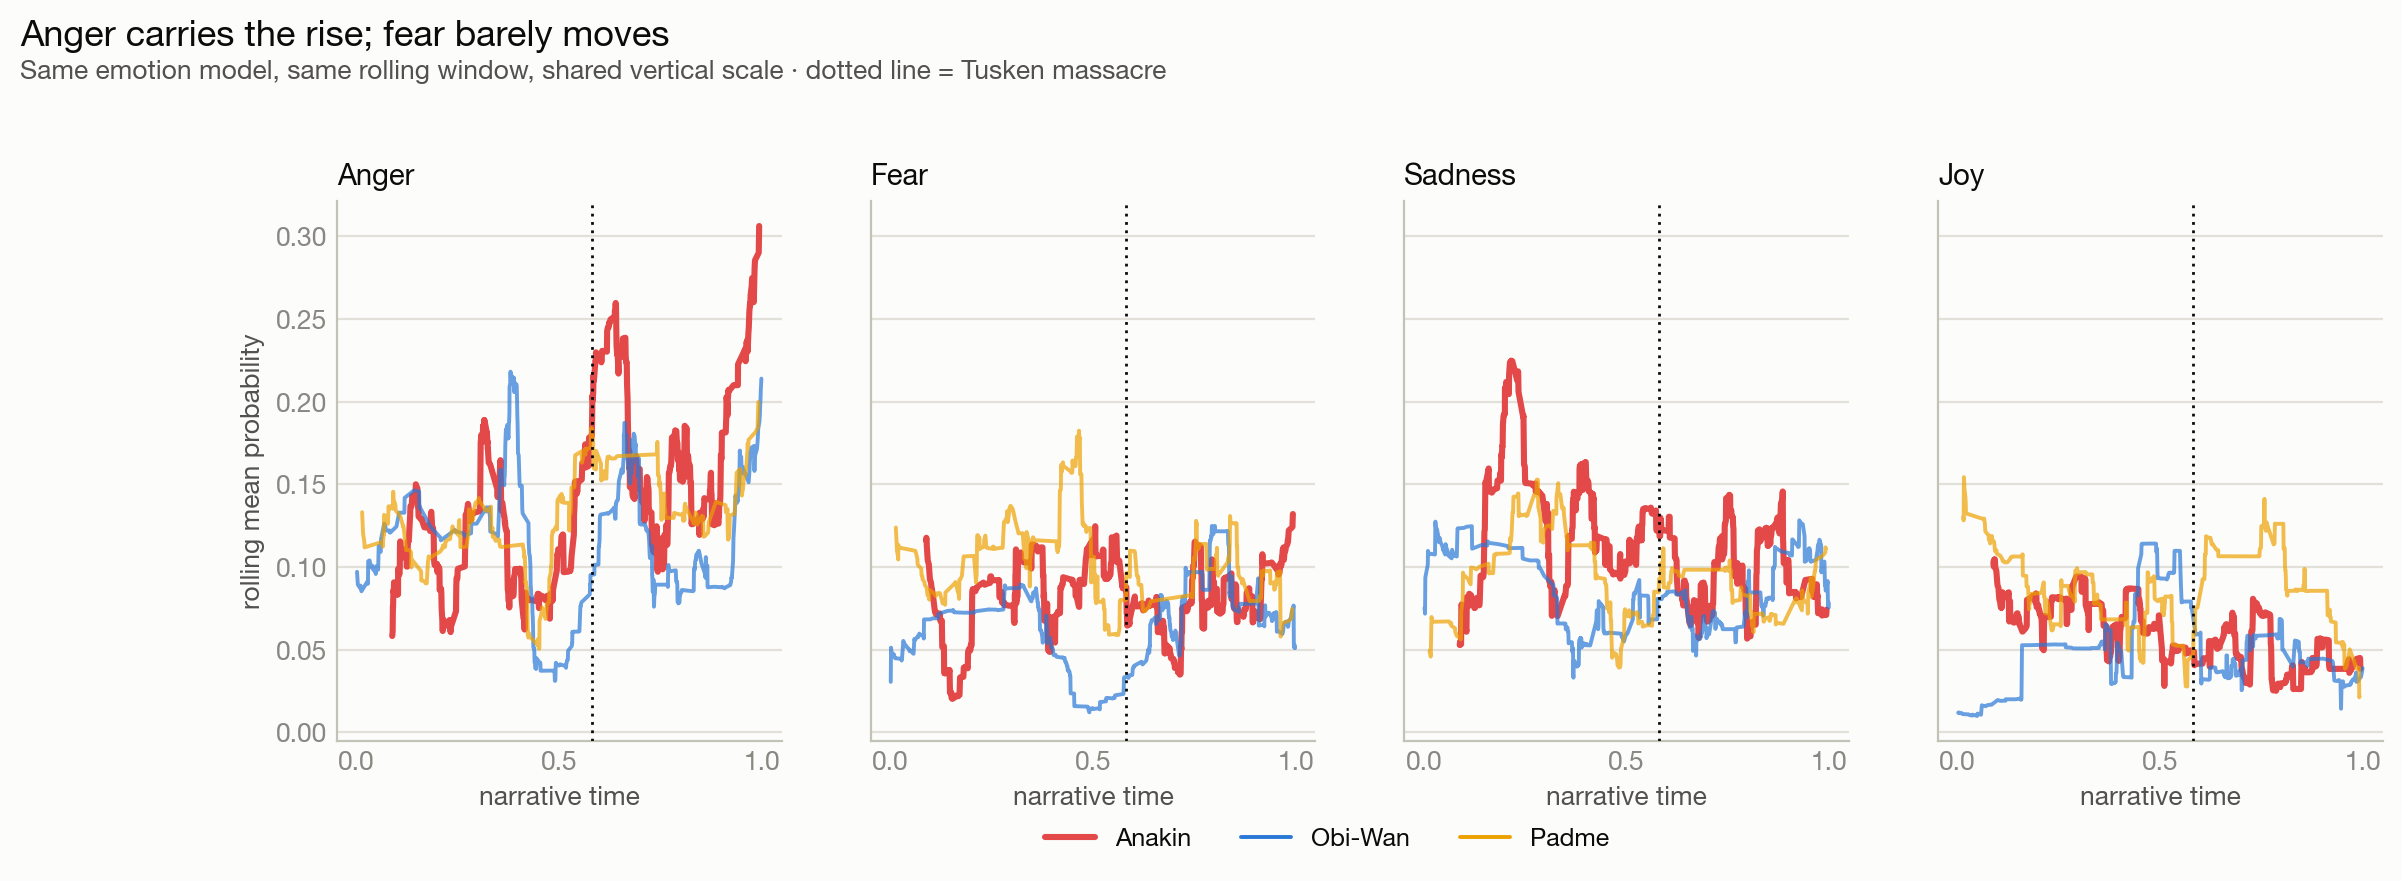
\includegraphics[width=0.96\linewidth]{../figures/03_emotion_panels.png}
\end{figure}

Surprise and joy fall more clearly than anger rises. Read this with care: most of the fall happens
between Episodes~I and~II, where the script source changes and the character goes from child to young
man. Inside Episodes~I and~II it is not significant. Question marks are part of the surprise score
(0.40 with one, 0.10 without), but removing those lines does not remove the fall ($\rho = -0.27$,
p $= 0.010$).

% ============================ 7 =============================================
\heading{7. Limitations}

\begin{itemize}
\setlength\itemsep{0.15em}
\item \textbf{Seven dark-side characters, and Palpatine has 52~\% of their lines.} That class is
      largely one voice, and this is the main constraint on the classifiers.
\item \textbf{Many tests on one small dataset.} Only the emotion table is adjusted for multiple
      comparisons, so isolated p-values near 0.05 are weak evidence.
\item \textbf{The three scripts differ in source and stage.} Episode~II is a revised draft, not a
      transcript. Changes between episodes can come from this, which makes comparisons within an
      episode more reliable.
\item \textbf{Story time is line rank, not screen time.} Scripts carry no timestamps.
\item \textbf{The models are out of domain and uncalibrated here,} so trends and contrasts mean more
      than absolute levels. Anakin's dark-side score and the controls' also come from models fitted
      on different training sets.
\end{itemize}

% ============================ 8 =============================================
\heading{8. Implementation}

The repository is a Python package (\texttt{src/anakin\_nlp/}) plus numbered scripts. The dataset has
2,940 lines from 64 characters, and 1,842 labelled lines from 26 characters train the classifiers.
\texttt{make all} reruns the pipeline, and every number in this report is in \texttt{reports/}.

The screenplays are third-party copyrighted works. The repository ships the code that fetches them,
not the texts: \texttt{data/} is git-ignored, and no figure, output or notebook cell reproduces
dialogue.

\end{document}
